\dev{Daphné Kany}{}

\textit{On présente l'utilité de la fenêtre glissante dans le protocole TCP : d'une part pour augmenter le taux d'envoi, et de l'autre pour réguler le trafic et éviter la congestion.}

\begin{com}
	On rappelle rapidement à l'orale l'existence du three way handshake précisé dans le plan. On se place ensuite directement au moment de l'échange de données.
\end{com}

\paragraph{Rappel}
\enspace\\
Alice et Bob communiquent en utilisant le protocole TCP. On suppose ici leur communication asymétrique : Alice envoie les données, Bob se contente de retourner les ACK. 

\begin{center}
	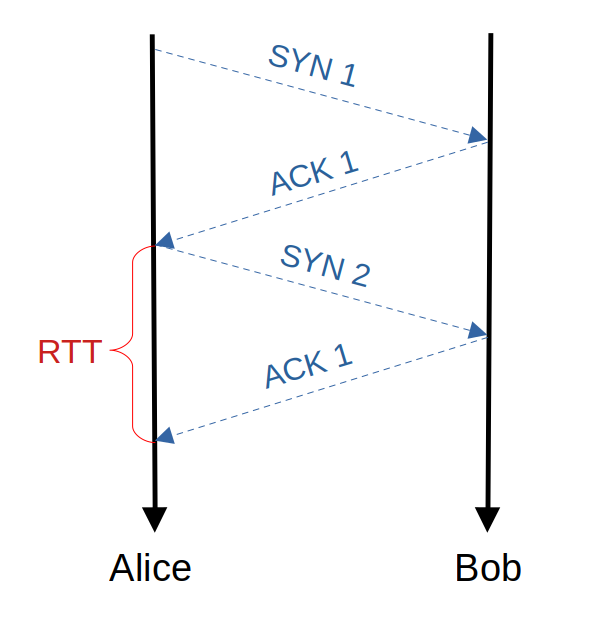
\includegraphics[height = 8cm]{Developpements/TCP/basique.png} \\
\end{center}

Quel est le taux d'envoi ? $\frac{1}{RTT}$. On voudrait améliorer ce taux. 

\paragraph{Solution 1 : Envoi en continu}
\enspace\\
Alice envoie tous les messages en continu. Problème : en cas d'erreur, Alice doit renvoyer le message et donc le garder en mémoire jusqu'à réception du ACK correspondant. Son buffer est limité. \\

\begin{center}
	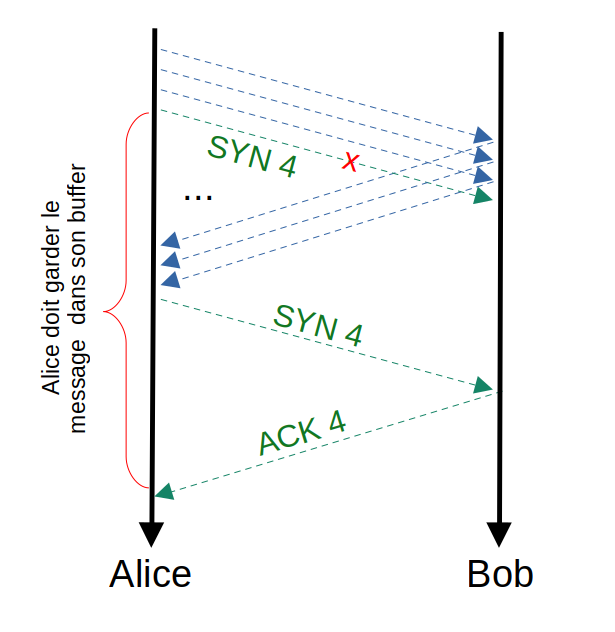
\includegraphics[height = 8cm]{Developpements/TCP/continu.png} \\
\end{center}

\paragraph{Solution 2 : La fenêtre glissante}
\enspace\\
On considère qu'Alice ne garde que $k$ messages dans son buffer. Lorsqu'il est plein, elle cesse d'envoyer. Dès qu'elle reçoit un ACK, elle supprime le message et en envoie un nouveau.

\begin{center}
	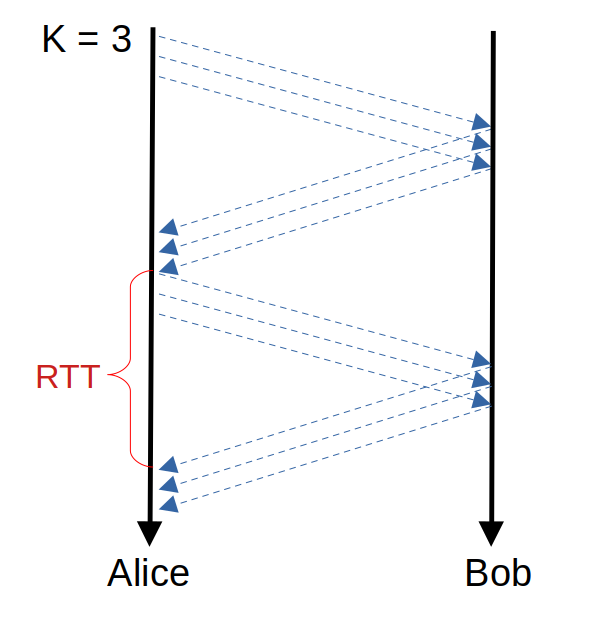
\includegraphics[height = 8cm]{Developpements/TCP/fenetre.png} \\
\end{center}

Taux d'envoi :  $\frac{k}{RTT}$
Comment déterminer la valeur de $k$ ? \\
Compromis entre le taux d'envoi et la taille du buffer d'Alice, et de ceux des routeurs sur le réseau pour éviter la congestion.

\begin{rem}
	Alice estime ici qu'il y a congestion si elle ne reçoit pas les ACK à temps. C'est en pratique assez vérifié pour les connexions fiables. 
\end{rem}

\begin{algorithm}[H]
	$k \gets 1$\\
	\Tq{il n'y a pas d'erreur}
	{Augmenter $k$}
	Recommencer
	\caption{Taille de la fenêtre glissante}
\end{algorithm}

A quelle vitesse augmenter $k$ ?

\paragraph{On l'augmente vite (exponentiellement)}
\enspace
\begin{com}
	Après tout c'est logique : on veut atteindre une grande valeur vite. Mais en fait, on n'en profite pas longtemps. 
\end{com}

\begin{center}
	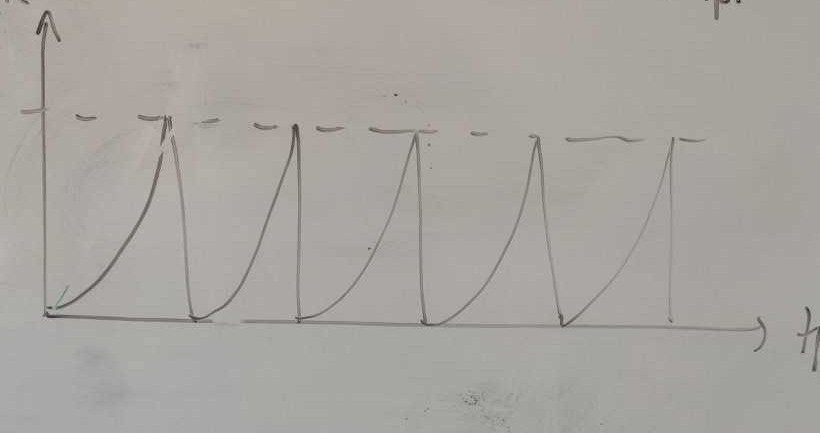
\includegraphics[width = 8cm]{Developpements/TCP/schema1.jpeg} \\
\end{center}

\paragraph{On l'augmente pas vite (linéairement)}
\enspace
\begin{com}
	C'est mieux. Mais on met du temps à atteindre le seuil. Combinons ces deux propositions :)
\end{com}

\begin{center}
	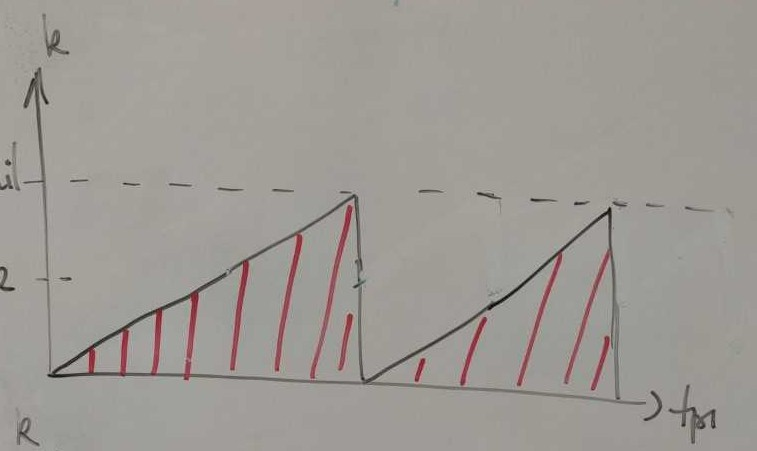
\includegraphics[width = 8cm]{Developpements/TCP/schema2.jpeg} \\
\end{center}

\paragraph{Combinons :)}
\enspace
\begin{com}
	Et beh quelle bonne idée. 
\end{com}
\begin{center}
	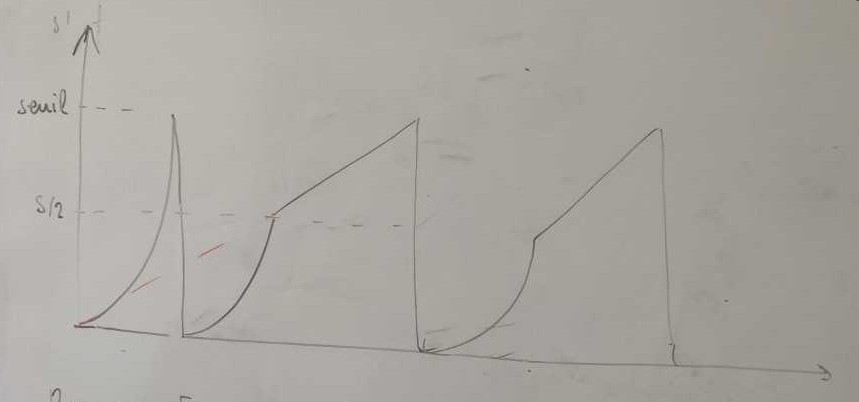
\includegraphics[width = 8cm]{Developpements/TCP/schema3.jpeg} \\
\end{center}

\paragraph{Et la descente ?}
\enspace\\
On peut aussi jouer sur la descente. On ne repart plus de k=1. 